\documentclass[main.tex]{subfiles}

\begin{document}

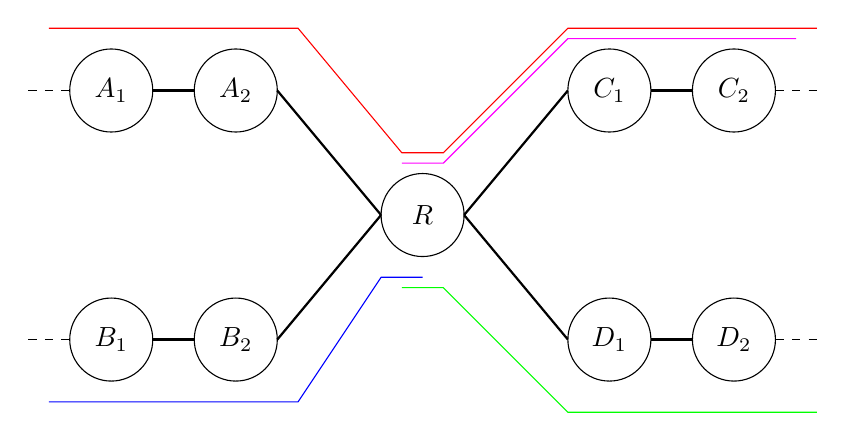
\begin{tikzpicture}[x=0.75pt,y=0.75pt,yscale=-1,xscale=1]

% begin part
\draw [dashed,black] (0, 60) -- (20, 60);
\draw (40, 60) circle (20) node {\texttt{$A_1$}};
\draw [fill opacity=1,thick,black] (60, 60) -- (80, 60);
\draw (100, 60) circle (20) node {\texttt{$A_2$}};

\draw [dashed,black] (0, 180) -- (20, 180);
\draw (40, 180) circle (20) node {\texttt{$B_1$}};
\draw [fill opacity=1,thick,black] (60, 180) -- (80, 180);
\draw (100, 180) circle (20) node {\texttt{$B_2$}};

\draw (190, 120) circle (20) node {\texttt{$R$}};
\draw [fill opacity=1,thick,black] (120, 60) -- (170, 120); 
\draw [fill opacity=1,thick,black] (120, 180) -- (170, 120); 
\draw [fill opacity=1,thick,black] (210, 120) -- (260, 60); 
\draw [fill opacity=1,thick,black] (210, 120) -- (260, 180); 

\draw (280, 60) circle (20) node {\texttt{$C_1$}};
\draw [fill opacity=1,thick,black] (300, 60) -- (320, 60);
\draw (340, 60) circle (20) node {\texttt{$C_2$}};
\draw [dashed,black] (360, 60) -- (380, 60);

\draw (280, 180) circle (20) node {\texttt{$D_1$}};
\draw [fill opacity=1,thick,black] (300, 180) -- (320, 180);
\draw (340, 180) circle (20) node {\texttt{$D_2$}};
\draw [dashed,black] (360, 180) -- (380, 180);

\draw [color={rgb, 255:red, 255; green, 0; blue, 0 }, draw opacity=1] (10, 30) -- ++ (120, 0) -- ++ (50, 60) -- ++ (20, 0) -- ++ (60, -60) -- ++ (120, 0);
\draw [color={rgb, 255:red, 0; green, 0; blue, 255 }, draw opacity=1] (10, 210) -- ++ (120, 0) -- ++ (40, -60) -- ++ (20, 0);
\draw [color={rgb, 255:red, 0; green, 255; blue, 0 }, draw opacity=1] (180, 155) -- ++ (20, 0) -- ++ (60, 60) -- ++ (120, 0);
\draw [color={rgb, 255:red, 255; green, 0; blue, 255 }, draw opacity=1] (180, 95) -- ++ (20, 0) -- ++ (60, -60) -- ++ (110, 0);
\end{tikzpicture}

\end{document}

